\section{{\maxIdletime}が一般の場合}
\label{section:LineArbitraryIdletime}

全点の{\maxIdletime}が等しい場合は,
結局巡査がそれぞれ独立な区間を一つずつ担当し往復する運行のみ考えればよいという
単純な状況になっていたが,
{\maxIdletime}が一般の場合は,
一部の点を複数の巡査が訪問して警邏する必要がある場合が存在する.
%
図\ref{tikz:multiAgentExample2}(左)の例では,
中央の{\maxIdletime}の短い二つの点は$2$人の巡査に訪問されており,
また,全点の{\maxIdletime}が等しい場合に反して
各巡査の最適な運行はなんらかの区間の往復であるとは限らないことも分かる.
%
また,
この例では左の巡査は左端の点を{\maxIdletime}ちょうどの間隔で訪問しているが,
一方,図\ref{tikz:multiAgentExample2}(中央)の例では,
左側の巡査は左端の点をあえてより短い周期で訪問することで全点を警邏している.
図\ref{tikz:multiAgentExample2}(中央)と同じ入力に対して,
図\ref{tikz:multiAgentExample2}(右)のように左の巡査が
左端の点の{\maxIdletime}ぎりぎりの時間まで右の方へ動き左端へ帰る運行を行うと
$2$人の巡査がうまく協力できず全点の警邏ができない.
このように,
補題\ref{lemm:LineUnaryIdletimeIndependentInterval}のときのように
左端の点の{\maxIdletime}から順に巡査の運行を決定することも難しい例が存在する.

\begin{figure}[htbp]
  \centering
  \begin{tabular}{ccc}
  \begin{minipage}{0.32\hsize}
    \centering
    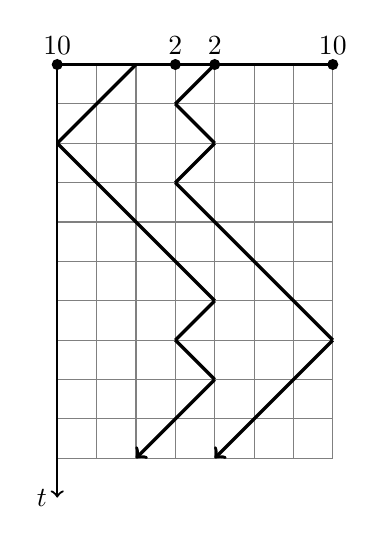
\begin{tikzpicture}
      \draw [help lines,thin,step=5mm] (0,-5.0) grid (3.5,0);
      \draw[thick] (0,0) -- (3.5,0) node [below] {};
      \draw[thick, ->] (0,0) -- (0,-5.5) node [left] {$t$};
      \fill ( 0   , 0) coordinate (c1) circle (2pt) node [above] {10};
      \fill ( 1.5 , 0) coordinate (c2) circle (2pt) node [above] {2};
      \fill ( 2.0 , 0) coordinate (c3) circle (2pt) node [above] {2};
      \fill ( 3.5 , 0) coordinate (c5) circle (2pt) node [above] {10};
      \draw[very thick,- ] ( 1.0, 0  )--(   0,-1.0);
      \draw[very thick,- ] (   0,-1.0)--( 2.0,-3.0);
      \draw[very thick,- ] ( 2.0,-3.0)--( 1.5,-3.5);
      \draw[very thick,- ] ( 1.5,-3.5)--( 2.0,-4.0);
      \draw[very thick,->] ( 2.0,-4.0)--( 1.0,-5.0);
      \draw[very thick,- ] ( 2.0, 0  )--( 1.5,-0.5);
      \draw[very thick,- ] ( 1.5,-0.5)--( 2.0,-1.0);
      \draw[very thick,- ] ( 2.0,-1.0)--( 1.5,-1.5);
      \draw[very thick,- ] ( 1.5,-1.5)--( 3.5,-3.5);
      \draw[very thick,->] ( 3.5,-3.5)--( 2.0,-5.0);
    \end{tikzpicture}
  \end{minipage}
  \begin{minipage}{0.32\hsize}
    \centering
    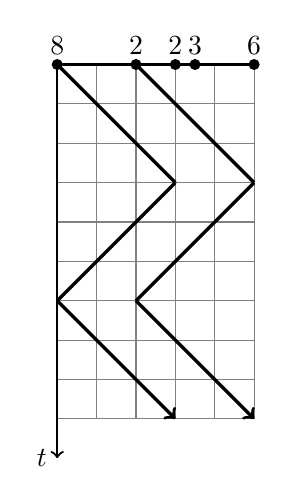
\begin{tikzpicture}
      \draw [help lines,thin,step=5mm] (0,-4.5) grid (2.5,0);
      \draw[thick] (0,0) -- (2.5,0) node [below] {};
      \draw[thick, ->] (0,0) -- (0,-5) node [left] {$t$};
      \fill ( 0   , 0) coordinate (c1) circle (2pt) node [above] {8};
      \fill ( 1   , 0) coordinate (c2) circle (2pt) node [above] {2};
      \fill ( 1.5 , 0) coordinate (c3) circle (2pt) node [above] {2};
      \fill ( 1.75, 0) coordinate (c4) circle (2pt) node [above] {3};
      \fill ( 2.5 , 0) coordinate (c5) circle (2pt) node [above] {6};
      \draw[very thick,- ] ( 0  , 0  )--( 1.5,-1.5);
      \draw[very thick,- ] ( 1.5,-1.5)--( 0  ,-3  );
      \draw[very thick,->] ( 0  ,-3  )--( 1.5,-4.5);
      \draw[very thick,- ] ( 1  , 0  )--( 2.5,-1.5);
      \draw[very thick,- ] ( 2.5,-1.5)--( 1  ,-3  );
      \draw[very thick,->] ( 1  ,-3  )--( 2.5,-4.5);
    \end{tikzpicture}
  \end{minipage}
  \begin{minipage}{0.32\hsize}
    \centering
    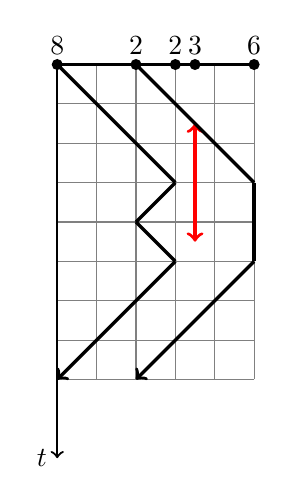
\begin{tikzpicture}
      \draw [help lines,thin,step=5mm] (0,-4) grid (2.5,0);
      \draw[thick] (0,0) -- (2.5,0) node [below] {};
      \draw[thick, ->] (0,0) -- (0,-5) node [left] {$t$};
      \fill ( 0   , 0) coordinate (c1) circle (2pt) node [above] {8};
      \fill ( 1   , 0) coordinate (c2) circle (2pt) node [above] {2};
      \fill ( 1.5 , 0) coordinate (c3) circle (2pt) node [above] {2};
      \fill ( 1.75, 0) coordinate (c4) circle (2pt) node [above] {3};
      \fill ( 2.5 , 0) coordinate (c5) circle (2pt) node [above] {6};
      \draw[very thick,red,<->] (1.75,-0.75)--(1.75,-2.25);
      \draw[very thick,- ] ( 0  , 0  )--( 1.5,-1.5);
      \draw[very thick,- ] ( 1.5,-1.5)--( 1  ,-2  );
      \draw[very thick,- ] ( 1  ,-2  )--( 1.5,-2.5);
      \draw[very thick,->] ( 1.5,-2.5)--( 0  ,-4  );
      \draw[very thick,- ] ( 1  , 0  )--( 2.5,-1.5);
      \draw[very thick,- ] ( 2.5,-1.5)--( 2.5,-2.5);
      \draw[very thick,->] ( 2.5,-2.5)--( 1  ,-4  );
    \end{tikzpicture}
  \end{minipage}
  \end{tabular}
  \caption{巡査の協力が必要な例.
    横軸を点の座標,縦軸を時刻として巡査の軌跡を表す.
    点の上の数値は{\maxIdletime}を表す.
    % \ncomment{[あとで図を差し替える]}
    \label{tikz:multiAgentExample2}}
\end{figure}


これらの例は,{\maxIdletime}が異なる場合は巡査の運行を個別に決定するのは難しいということを示唆している.
しかしながら,
地図が{\graphLine}で{\maxIdletime}が一般の場合での{\PPProfit}の困難性を示すこともできなかった.
そこで,{\maxIdletime}より短い間隔で点を訪問しうることで運行の決定が複雑になる例が存在したことを踏まえて,
ここでは\ref{chapter: introduction}章で定義した別種の問題,{\timeSpecifiedPP}を代わりに考える.


地図が{\graphLine}の場合の{\timeSpecifiedPP}は,
正の整数$m$と
$n$個の自然数の組$(q_i, r_i, x_i)_{ i \in \{ 1, \ldots, n \} }$が与えられたとき,
集合
$\{ (q_i k + r_i, x_i) \mid k \in \Zset, i \in \{1, \ldots, n\} \}$を
$m$個以下の運行可能集合に分割できるか判定する問題と言い換えることができる.
%
ただし,
集合$S \subset \Zset \times \Zset$が\defword{運行可能}であるとは,
任意の$(t_1, x_1), (t_2, x_2) \in S$が
$\abs{x_1 - x_2} \leq \abs{t_1 - t_2}$を満たすことであり,
分割$\{ P_1, \ldots, P_h \}$が\defword{運行可能}であるとは,
$P_1, \ldots, P_h$がそれぞれ運行可能であることと定義する.
% \ncomment{[運行可能分割の説明の図]}
%
任意の運行可能集合$S$に対して,
{\graphLine}上の巡査の運行$a$であって,
$S$のすべての元$(t, x)$に対して$a(t) = x$を満たす
(このとき$a$を運行可能集合$S$に対応する運行と呼ぶ)
ものが存在することは簡単に示すことができる.



まず,地図が{\graphLine}の場合は順序保存運行を考えることができるのと同様に,
順序保存(運行可能)分割を考えることができる.
分割$\mathcal{P} = \{ P_1, \ldots, P_h \}$が\defword{順序保存}であるとは,
$\mathcal{P}$に対応する運行$A = (a_1, \ldots, a_h)$であって
順序保存なものが存在すること,
あるいは,
\begin{align*}
  L(t, x)
    &:= \{ (t', x') \mid
          \abs{x - x'} > \abs{t - t'} \;\textrm{かつ}\; x' < x \} \\
    &= \{ (t', x') \mid {x - x'} > \abs{t - t'} \}
\end{align*}
として,
任意の$P_i\ (i \in \{ 1 \ldots, h \})$について,
領域$\bigcup_{(t, x) \in P_i} L(t, x)$に
$P_j\ (i < j)$の点が存在しないことと定義する.
% \ncomment{[$L$の説明の図]}

\newcommand{\minpart}{\mathfrak{P}}

$X := \{ (q_i k + r_i, x_i) \mid k \in \Zset, i \in \{1, \ldots, n\} \}$の
任意の順序保存分割のうち一番左の集合は順序保存分割の定義から
$\minpart_1 := \{ (t, x) \in X \mid L(t, x) \cap X = \emptyset \}$の
部分集合となる.
よって,$X$の最小の順序保存分割であって一番左の集合が
$\minpart_1$であるようなものが存在する.
%
同様に,残りの$X \setminus \minpart_1$の最小の順序保存分割であって一番左の集合が
$\minpart_2 :=
  \{ (t, x) \in X \setminus \minpart_1
      \mid L(t, x) \cap X \setminus \minpart_1 = \emptyset \}$であるようなものが存在する.
このように,集合$X$の左側から貪欲に運行可能集合を取り出していく操作を再帰的に繰り返すと,
最小の順序保存分割$\{ \minpart_1, \minpart_2, \ldots, \minpart_h \}$が得られる.
これを$\minpart(X)$と書くことにする.
全点を定時訪問する運行が存在するには,
$\card{\minpart(X)} \leq m$が成り立つことが必要十分である.

\newcommand{\subsegment}[3]{{#1}_{[#2:#3)}}
以下では,集合$S \subseteq \Zset \times \Zset$に対して
$\subsegment{S}{a}{b} := \{ (t, x) \in S \mid a \leq t < b \}$と定義する.

$q_1, \ldots, q_n$が整数であるので
$X$は時刻(組$(t, x) \in X$の第1要素)について周期的であり,
その周期は$q_1, \ldots, q_n$の最小公倍数$T$となる
(すなわち,任意の整数$k$に対して,
$(t, x) \in \subsegment{X}{kT}{(k + 1)T}$と$(t - kT, x) \in \subsegment{X}{0}{T}$が同値である).
従って,前述の貪欲な分割$\minpart(X)$の各要素
$\minpart_i\ (i \in \{1, \ldots, h \})$も同様に時刻について周期的である
(すなわち,任意の$\minpart_i$と整数$k$に対して,
$(t, x) \in \subsegment{\minpart_i}{kT}{(k + 1)T}$と
$(t - kT, x) \in \subsegment{\minpart_i}{0}{T}$が同値である).
%
よって,
$X$の最小の運行可能分割
$\minpart(X) = \{ \minpart_1, \ldots, \minpart_h \}$の大きさを知るには,
$\subsegment{X}{0}{T}$の運行可能分割
$\{ \subsegment{\minpart_1}{0}{T}, \ldots, \subsegment{\minpart_h}{0}{T} \}$を計算すれば十分である.

ここで,$\minpart(\subsegment{X}{0}{T})$と$\minpart(X)$の大きさは
必ずしも一致しないことに注意する必要がある.
前述の貪欲な分割の仕方で集合$S$から左端の運行可能集合
$s' := \{ (t, x) \in S \mid L(t, x) \cap S = \emptyset \}$を取り出すとき,
$s'$の点$(t, x)$の条件は領域$L(t, x)$に$S$の点が存在しないことである.
$X$の分割$\minpart(X) = \{ \minpart_1, \ldots, \minpart_h \}$%
の部分となるような$\subsegment{X}{0}{T}$の分割
$\{ \subsegment{\minpart_1}{0}{T}, \ldots, \subsegment{\minpart_h}{0}{T} \}$
を得るには,
$\subsegment{X}{0}{T}$のいずれかの点$(t, x)$に対して
$L(t, x)$に含まれるような$X$の点全体,すなわち
$X \cap \bigcup_{(t, x) \in \subsegment{X}{0}{T}}L(t, x)$%
を含む集合$F$を分割する必要がある.
$\minpart(F)$の各要素を$[0:T)$に制限すれば
$\{ \subsegment{\minpart_1}{0}{T}, \ldots, \subsegment{\minpart_h}{0}{T} \}$%
が得られる.
$F$は例えば
$W = \max(x_1, \ldots, x_n) - \min(x_1, \ldots, x_n)$%
として
$\{ (t, x) \in X \mid -W \leq t \leq T + W \}$%
とすればよい.


以上の議論から,
地図$(U, V)$が{\graphLine}の場合の{\timeSpecifiedPP}は
以下の貪欲アルゴリズムで解くことができる.

$V = \{ x_1, \ldots, x_n \}$とし,
$x_i \in V$の{\exactTime}を$(q_i, r_i)$とする.

$W = \max(V) - \min(V)$を計算する.
%
\[
  F = \{ (q_i k + r_i, x_i) \mid
    i \in \{ 1, \ldots, n \},
    k \in \Zset, -W \leq q_i k + r_i < T + W \}
\]
を求める.
{\setPartAlgo}の入力として$F$を与え,
出力$\mathcal{P}$について$\card{\mathcal{P}} \leq m$であるかどうかを判定する.

\begin{setPartitionAlgorithm}
  入力を有限集合$S$とする.
  初期値を$\mathcal{P} = \{\}$, $S' = S$とし,
  $S' \neq \emptyset$である限り
  次の(\ref{item:alg_step_first})から(\ref{item:alg_step_last})を繰り返す.
  \begin{enumerate}[(i)]
  \item \label{item:alg_step_first}
    $P \gets \{ (t, x) \in S' \mid L(t, x) \cap S' = \emptyset \}$
  \item
    $\mathcal{P} \gets \mathcal{P} \cup \{ P \}$
  \item \label{item:alg_step_last}
    $S' \gets S' \setminus P$
  \end{enumerate}
  $\mathcal{P}$を出力する.
\end{setPartitionAlgorithm}


% {\setPartAlgo}は,
% 有限集合$A$の分割$\minpart(A)$を与えるアルゴリズムであり,
% 出力された分割$\mathcal{P}$の各要素を$[0:T)$に制限すれば
% $\subsegment{X}{0}{T}$の分割$\{ \subsegment{\minpart_1}{0}{T}, \ldots, \subsegment{\minpart_h}{0}{T} \}$が得られる.
